\documentclass{beamer}
\usepackage{graphicx}
\usepackage{graphics}
\usepackage{hyperref}
\usepackage[english]{babel}
\usepackage[T1]{fontenc}
\usepackage[utf8]{inputenc}
\usepackage{xfrac}
\usepackage{array}
\usepackage{multirow}
\usepackage[normalem]{ulem}


\mode<presentation>
{
    \usetheme{AMUFree-kk}
    \setbeamercovered{transparent = 28}
}
\title{Training MLM models without softmax distribution}
\date{2023}
\author{Karol Kaczmarek}
\setbeamertemplate{bibliography item}{[\theenumiv]}


\begin{document}

\begin{frame}
    \titlepage
\end{frame}

\iffalse
\AtBeginSection[]
{
    \begin{frame}
        \frametitle{Outline}
        \tableofcontents[currentsection]
    \end{frame}
}
\fi

\begin{frame}
    \frametitle{Predicting Next Tokens - CLM}
    \begin{center}
        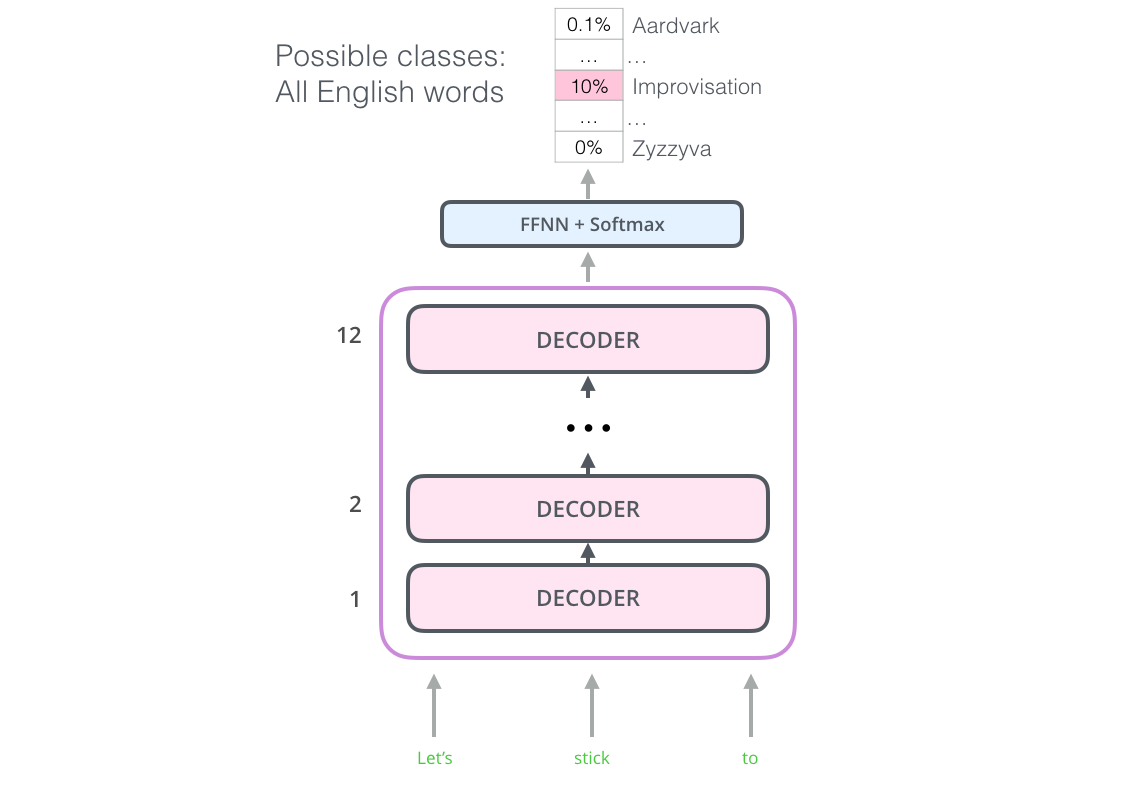
\includegraphics[scale=0.2]{img/clm.png}
    \end{center}
     \tiny Image from: \href{https://jalammar.github.io/illustrated-bert/}{The Illustrated BERT, ELMo, and co. (How NLP Cracked Transfer Learning)}
\end{frame}

\begin{frame}
    \frametitle{Predicting Masked Tokens - MLM}
    \begin{center}
        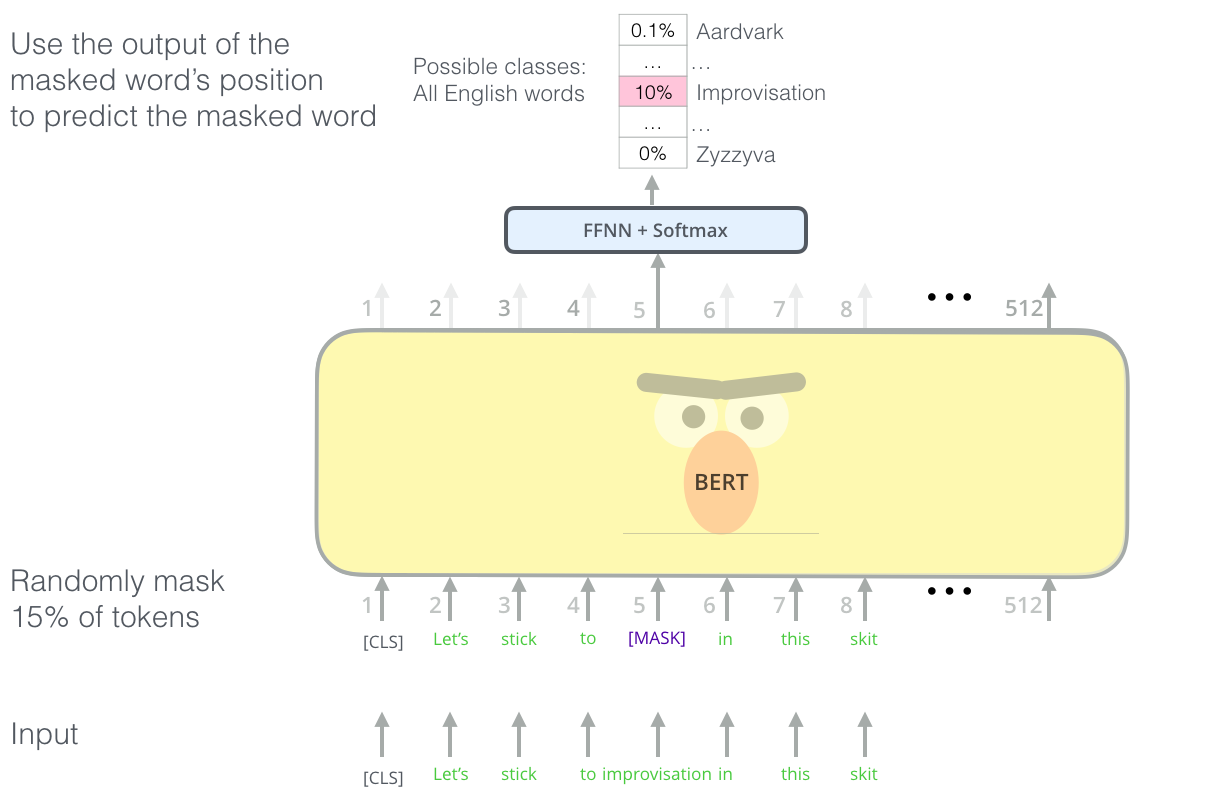
\includegraphics[scale=0.2]{img/mlm.png}
    \end{center}
     \tiny Image from: \href{https://jalammar.github.io/illustrated-bert/}{The Illustrated BERT, ELMo, and co. (How NLP Cracked Transfer Learning)}
\end{frame}

\begin{frame}
    \frametitle{T64 (2018) \cite{t64}}
    \begin{center}
        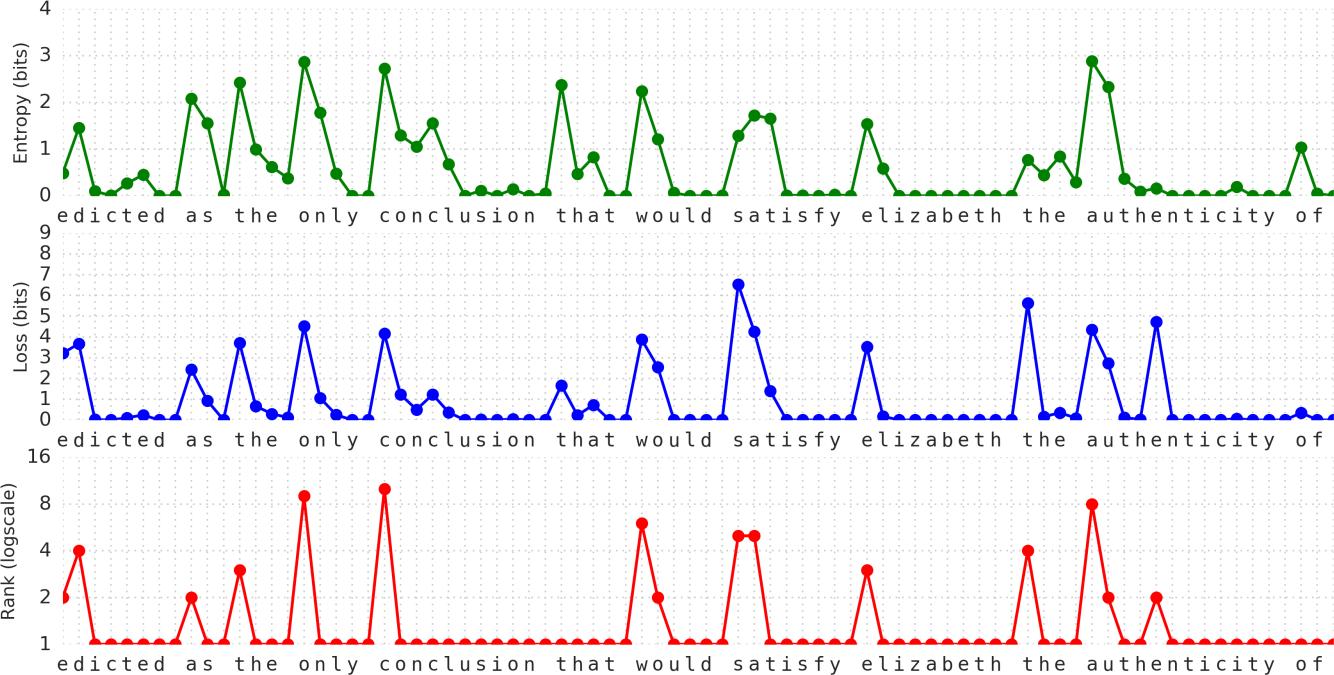
\includegraphics[scale=1.0]{img/t64.png}
    \end{center}
\end{frame}

\begin{frame}
    \frametitle{Charformer (2021) \cite{charformer}}
    \begin{center}
        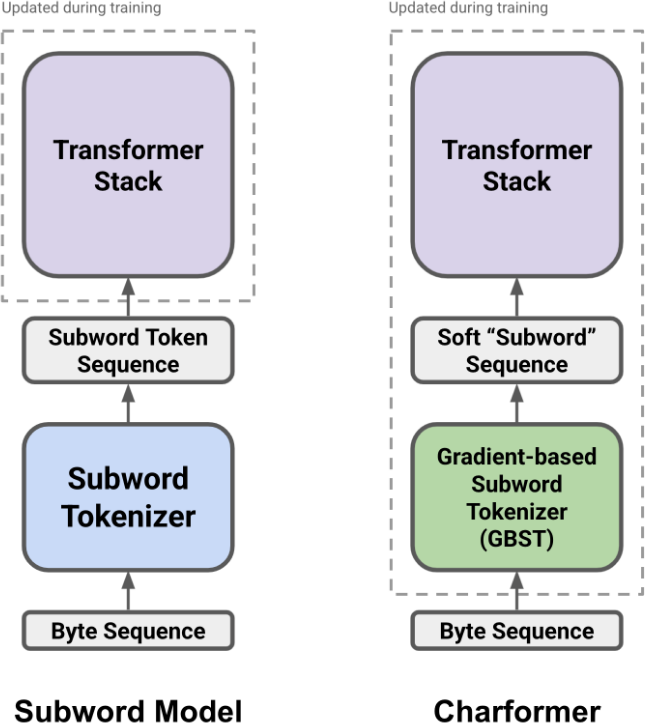
\includegraphics[scale=1.0]{img/gbst.png}
    \end{center}
\end{frame}

\begin{frame}
    \frametitle{GPT-2 (2019) \cite{gpt2} - Byte BPE}
    \begin{center}
        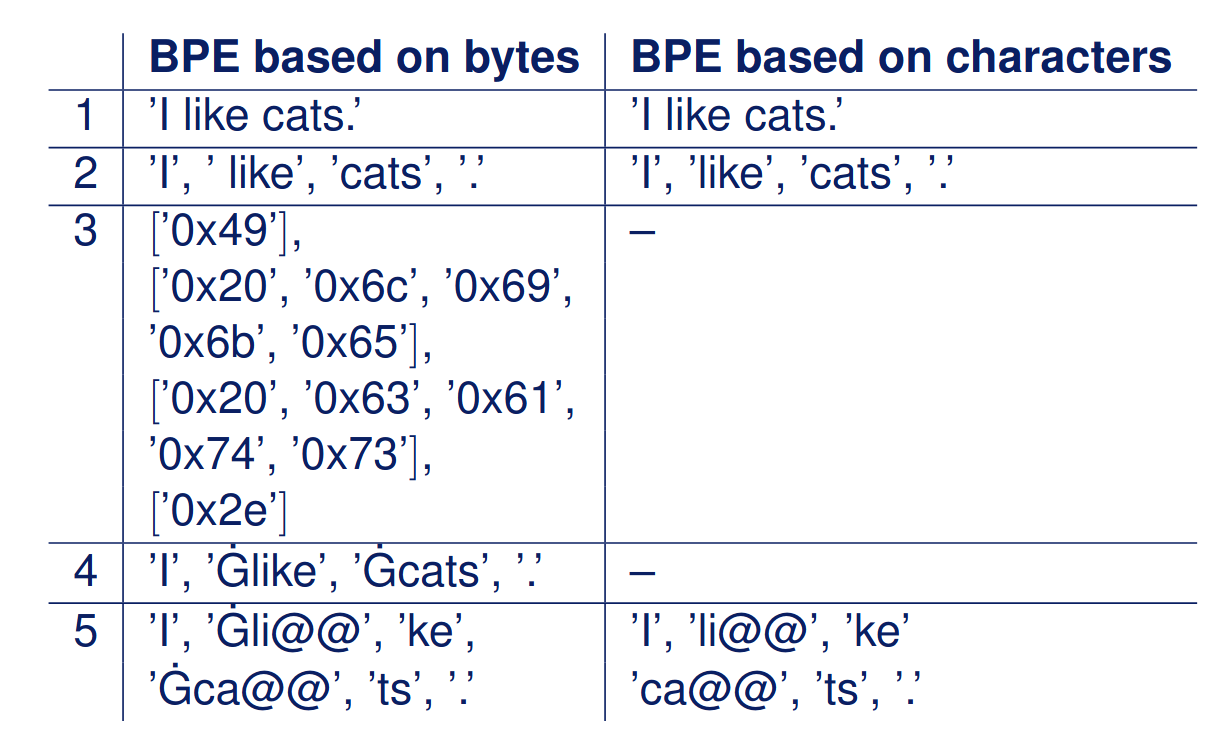
\includegraphics[scale=0.25]{img/byte-bpe-1.png}
    \end{center}
\end{frame}

\begin{frame}
    \frametitle{XLM-RoBERTa (2019) \cite{xlmr} / mT5 (2020) \cite{mt5}}
    \begin{center}
        XLM-RoBERTa:
        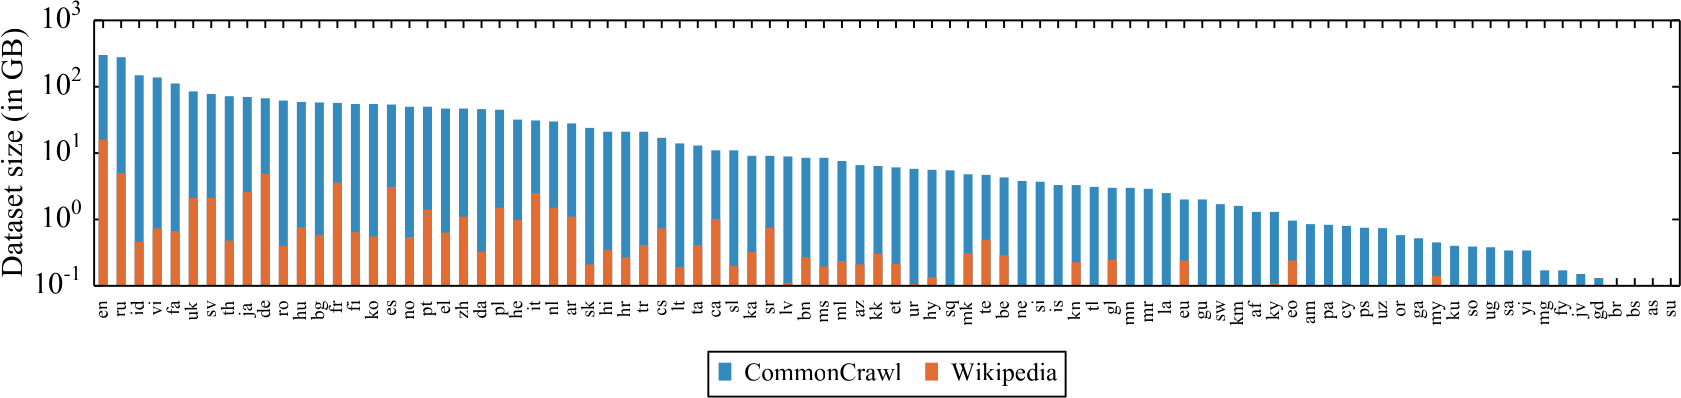
\includegraphics[scale=0.8]{img/xlmr.png}
        mT5:
        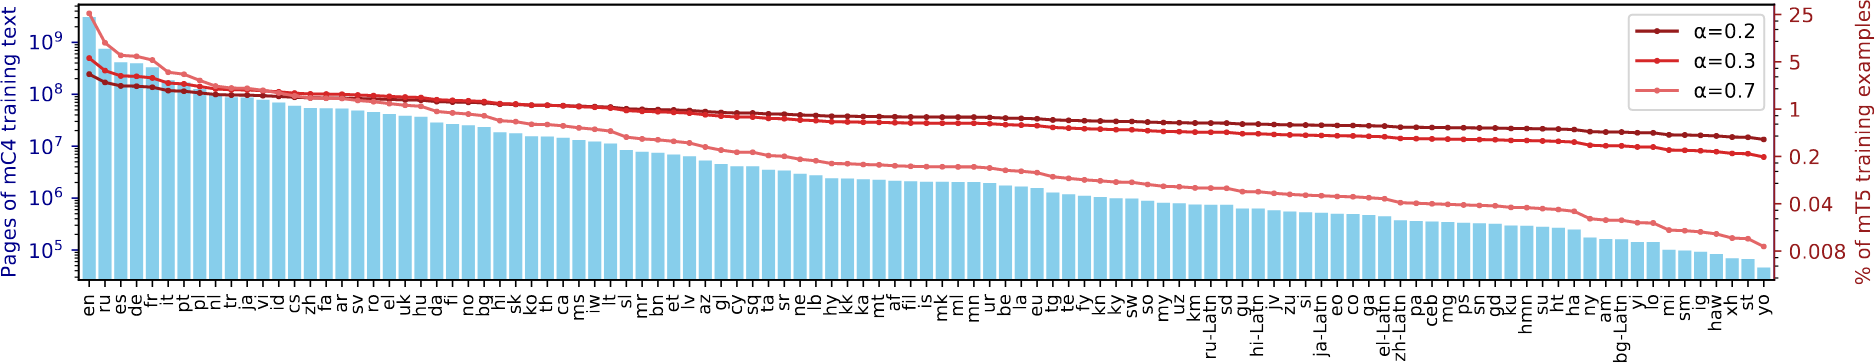
\includegraphics[scale=0.75]{img/mt5.png}
    \end{center}
\end{frame}

\begin{frame}
    \frametitle{ByT5 (2021) \cite{byt5}}
    \begin{center}
        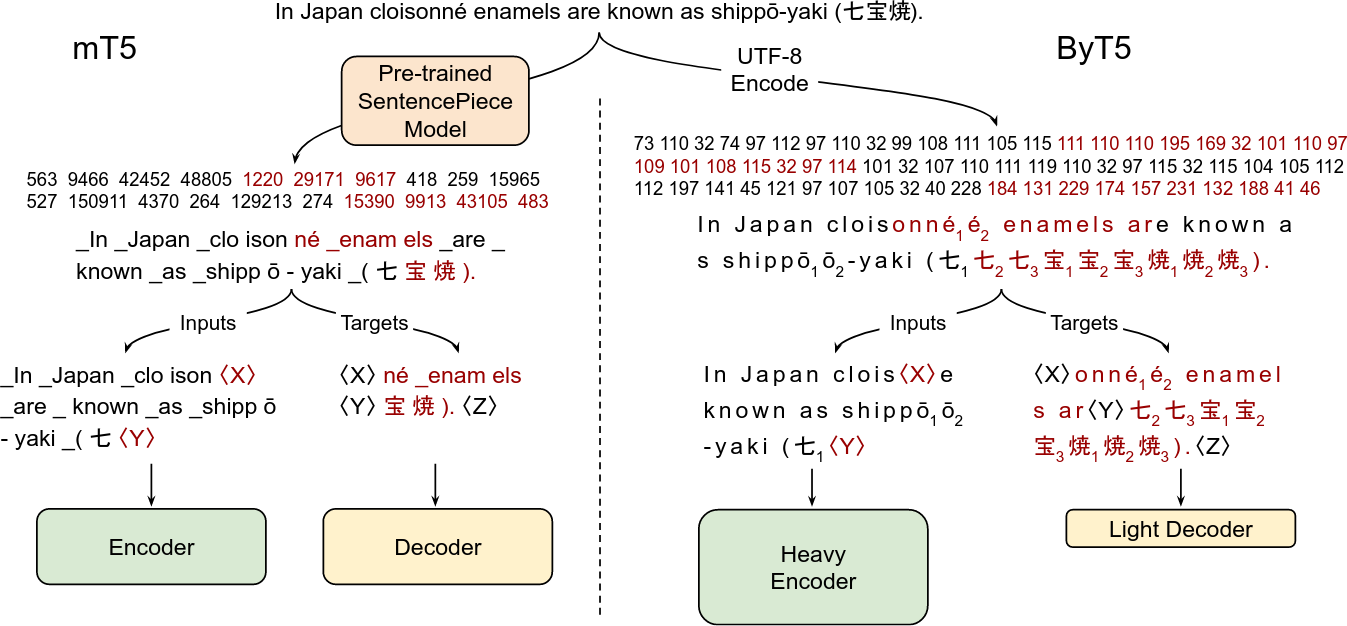
\includegraphics[scale=1.0]{img/mt5_and_byt5.png}
    \end{center}
\end{frame}

\begin{frame}
    \frametitle{Visual Text Representation (2021) \cite{vtr_emb}}
    \begin{center}
        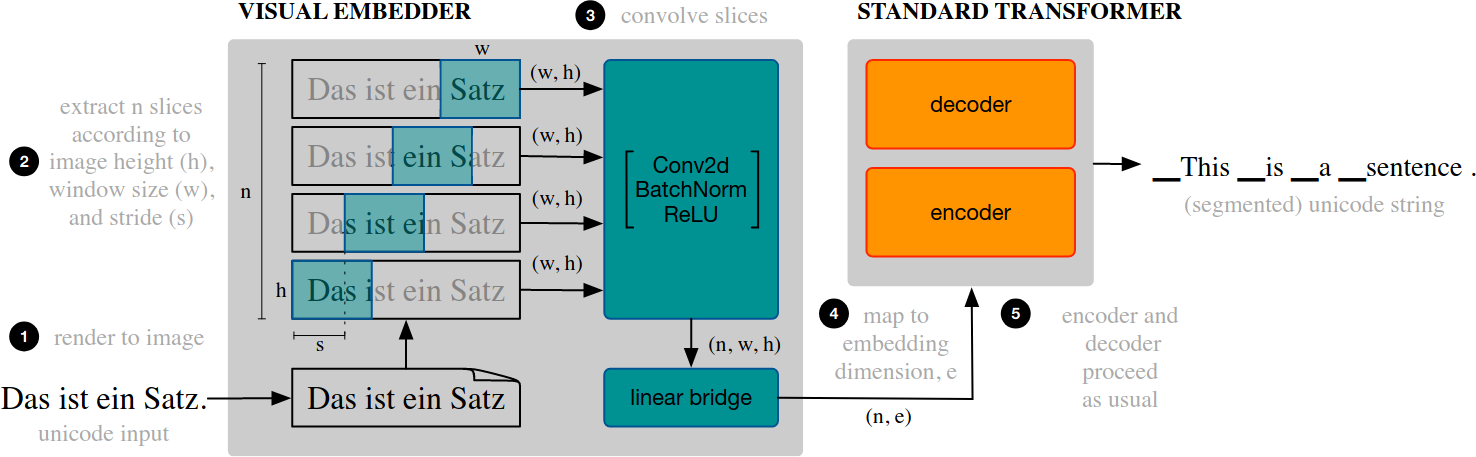
\includegraphics[scale=0.95]{img/vtr_emb.png}
    \end{center}
\end{frame}

\begin{frame}
    \frametitle{\textbf{N}on\textbf{P}arametric \textbf{M}asked Language Model (NPM) \cite{nonparametric_mlm}}
    \begin{itemize}
        \item December 2023, MetaAI - PyTorch (with code release: \href{https://github.com/facebookresearch/NPM}{GitHub})
        \item predicts tokens based on a nonparametric distribution over phrases in a text corpus
        \item does not have a softmax over a fixed output vocabulary
        \item nonparametric distribution is defined by a function of the available data, not by a fixed set of parameters (LM-Head)
        \item predict extremely rare, unseen words and disambiguating word senses
        \item support effectively unlimited vocabulary sizes
    \end{itemize}
\end{frame}

\begin{frame}
    \frametitle{Illustration of NPM}
    \begin{center}
        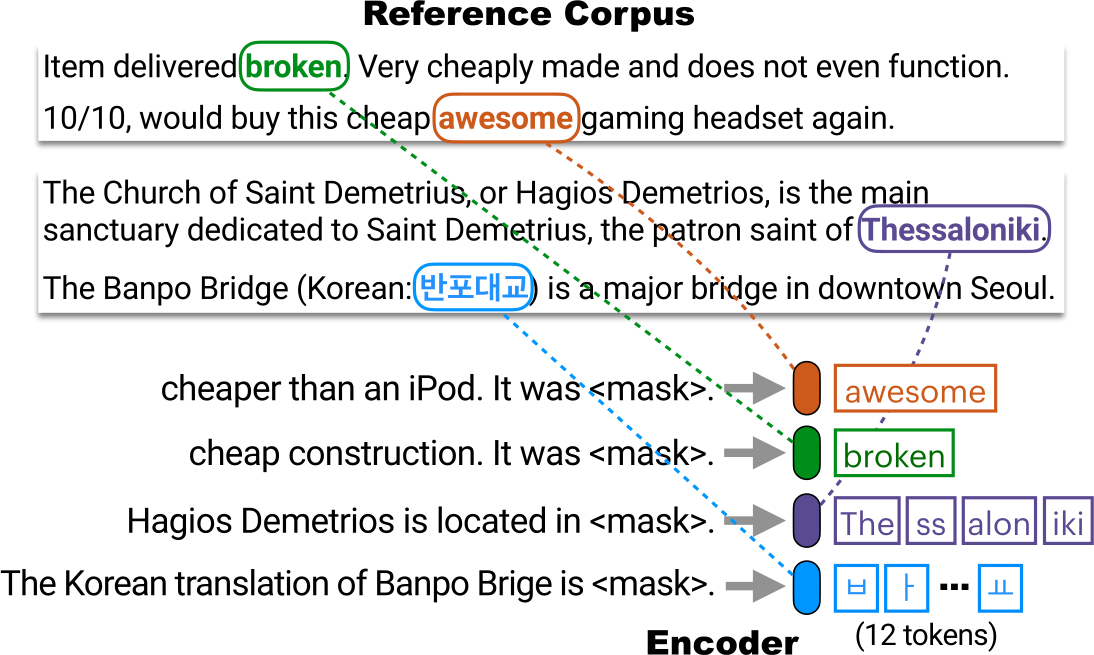
\includegraphics[scale=0.58]{img/npm1.png}
    \end{center}
    \begin{itemize}
        \footnotesize
        \item NPM consists of an \textbf{encoder} and a \textbf{reference corpus}, and models a \textbf{nonparametric distribution} over a reference corpus
        \item key idea is to \textbf{map all the phrases in the corpus into a dense vector space} using the encoder
        \item at inference when given a query with a <MASK>, use the encoder to \textbf{locate the nearest phrase from the corpus} and \textbf{fill in the <MASK>}
        \item NPM can fill with \textbf{multiple tokens}
    \end{itemize}
\end{frame}

\begin{frame}
    \frametitle{Mapping phrase into dense vector space}
    \begin{center}
        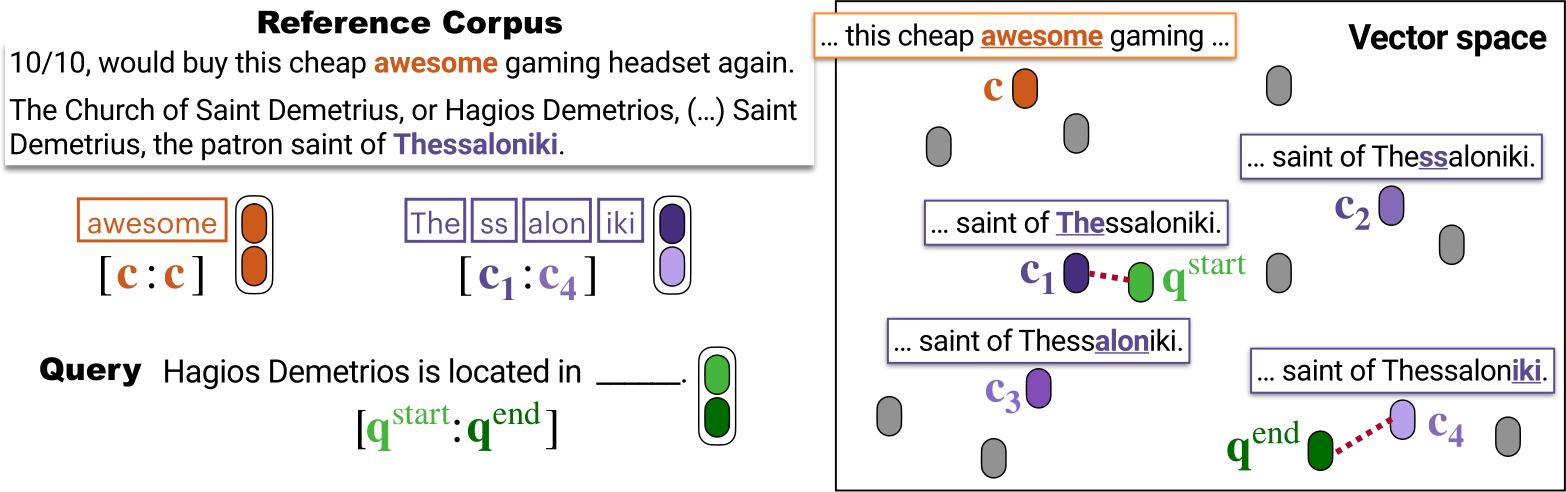
\includegraphics[scale=0.6]{img/npm2.png}
    \end{center}
    \begin{itemize}
        \footnotesize
        \item encoder maps \textbf{every distinct phrase} in a reference corpus into a \textbf{dense vector space}
        \item standard indexing is expensive (indexing each token)
        \item represents a phrase with a \textbf{concatenation} of the token representation of the \textbf{start} and the \textbf{end} of the phrase
        \item phrase consisting of 4 BPE tokens $c_1$, $c_2$, $c_3$, $c_4$ is represented with a concatenation of vectors of $c_1$ and $c_4$
    \end{itemize}
\end{frame}

\begin{frame}
    \frametitle{Retrieving phase}
    \begin{center}
        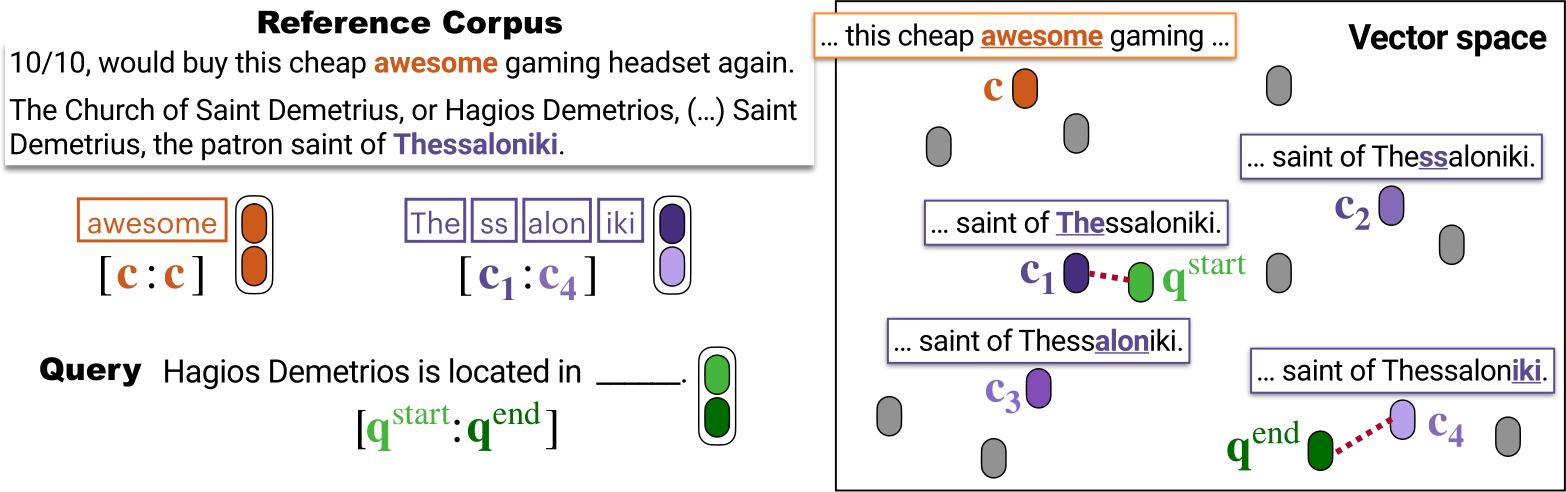
\includegraphics[scale=0.6]{img/npm2.png}
    \end{center}
    \begin{itemize}
        \footnotesize
        \item replace <MASK> token to <MASK$_{s}$> and <MASK$_{e}$> tokens (representing the start and the end of the phase)
        \item replace each of token to vectors with the same vector space, respectively: $q^{start}$ and $q^{end}$ vectors
        \item use these vectors to \textbf{retrieve the start and the ending of the phrases}
    \end{itemize}
    \begin{center}
    $ q_{1}, ..., q_{t-1}, q^{start}, q^{end}, q_{t+2}, ..., q_{L} = Encoder (t_{1}, ..., t_{t-1}, MASK_{s}, MASK_{e}, t_{t+2}, ..., t_{L}) $
    \end{center}
\end{frame}

\begin{frame}
    \frametitle{Approximation}
    \begin{center}
        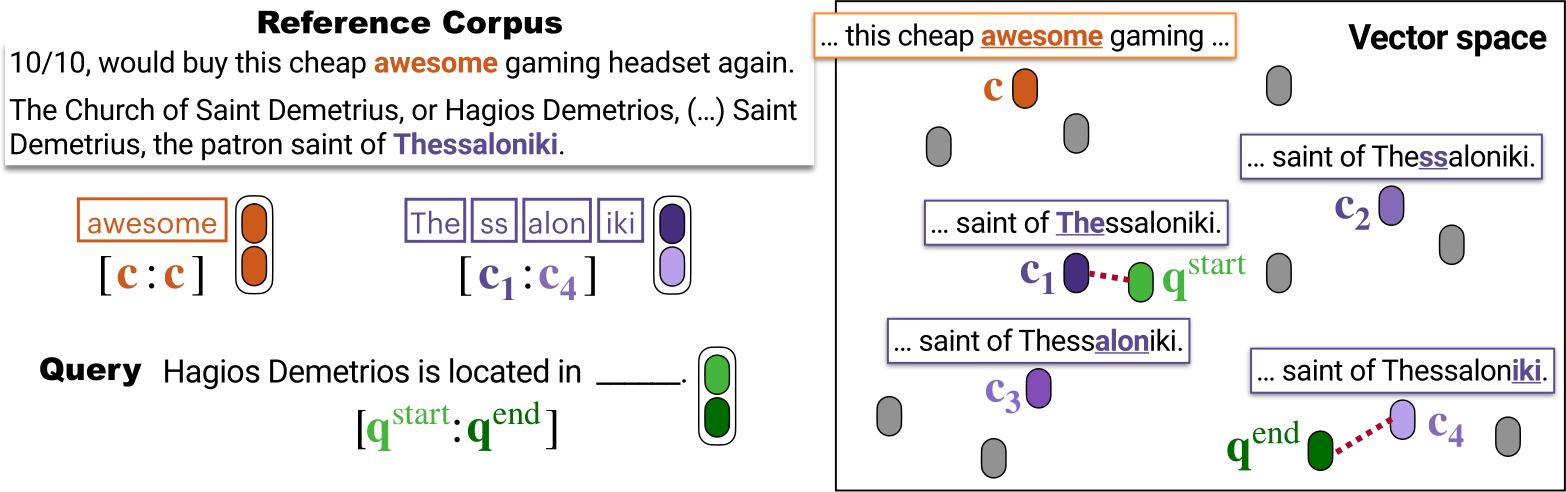
\includegraphics[scale=0.8]{img/npm2.png}
    \end{center}
    \begin{itemize}
        \footnotesize
        \item in practice, iterating over all phrases from corpus is infeasible
        \item approximation: using a fast nearest neighbor search for the start and the end separately -- \textbf{take the top-k tokens with the highest
similarity scores} with each of them, and \textbf{compute
scores over spans composed by these tokens}
        \item use \textbf{scaled inner product} as similarity function
    \end{itemize}
\end{frame}

\begin{frame}
    \frametitle{Training - issues}
    \begin{enumerate}
        \footnotesize
        \item full corpus retrieval can make training very expensive
        \begin{itemize}
            \item in-batch approximation to a full corpus -- removing the need for keeping and updating the retrieval index during training
        \end{itemize}

        \item filling in a <MASK> with an arbitrary length phrase instead of a token is non-trivial
        \begin{itemize}
            \item extensions to span masking and a contrastive objective which allow filling a <MASK> with a phrase
        \end{itemize}
    \end{enumerate}
\end{frame}

\begin{frame}
    \frametitle{Masking}
    \begin{center}
        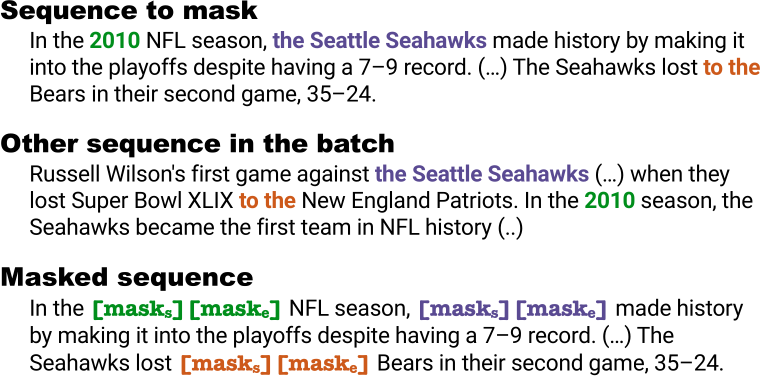
\includegraphics[scale=1.15]{img/npm4.png}
    \end{center}
    \begin{enumerate}
        \footnotesize
        \item mask spans if they co-occur in the other sequences in the batch
        \begin{itemize}
            \item masked tokens: \textbf{2012} and \textbf{the Seattle Seahawks} and \textbf{to the}
            \item \textbf{second game} will not used because \textbf{second} and \textbf{game} do not occur together in the other sequence in the batch
        \end{itemize}
        \item replace the whole span with two special tokens: <MASK$_s$> and <MASK$_e$>
    \end{enumerate}
\end{frame}

\begin{frame}
    \frametitle{Training Object -- contrastive learning}
    \begin{center}
        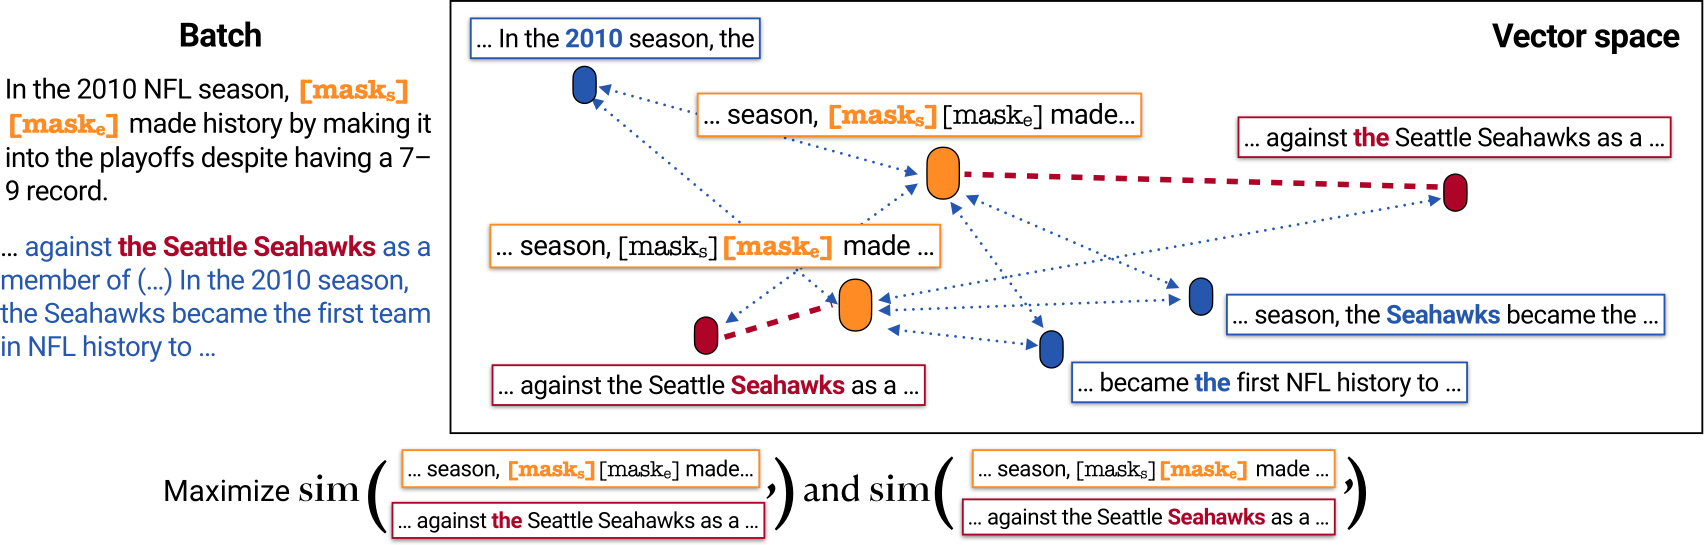
\includegraphics[scale=0.79]{img/npm3.png}
    \end{center}
    \begin{itemize}
        \footnotesize
        \item model should retrieve a phrase \textbf{the Seattle Seahawks} from other sequences in the reference corpus
        \item MASK$_{s}$ vector should be closer to \textbf{the Seattle Seahawks} (\textbf{positive sample}) while being distant from other tokens and should not be any \textbf{the} (from \textbf{became the first} -- \textbf{negative sample}), similar to MASK$_{e}$ vector
    \end{itemize}
\end{frame}

\begin{frame}
    \frametitle{Training Details}
    \begin{itemize}
        \item corpus: English Wikipedia and English portion of CC-News -- contains 13B tokens in total
        \item segmented into sequences, each with up to 256 tokens
        \item initialize from RoBERTa large
        \item training: 100 000 steps, 32 x 32GB GPUs
        \item one batch consists of 512 sequences
GPUs
    \end{itemize}
\end{frame}

\begin{frame}
    \frametitle{Scores}
    \begin{center}
        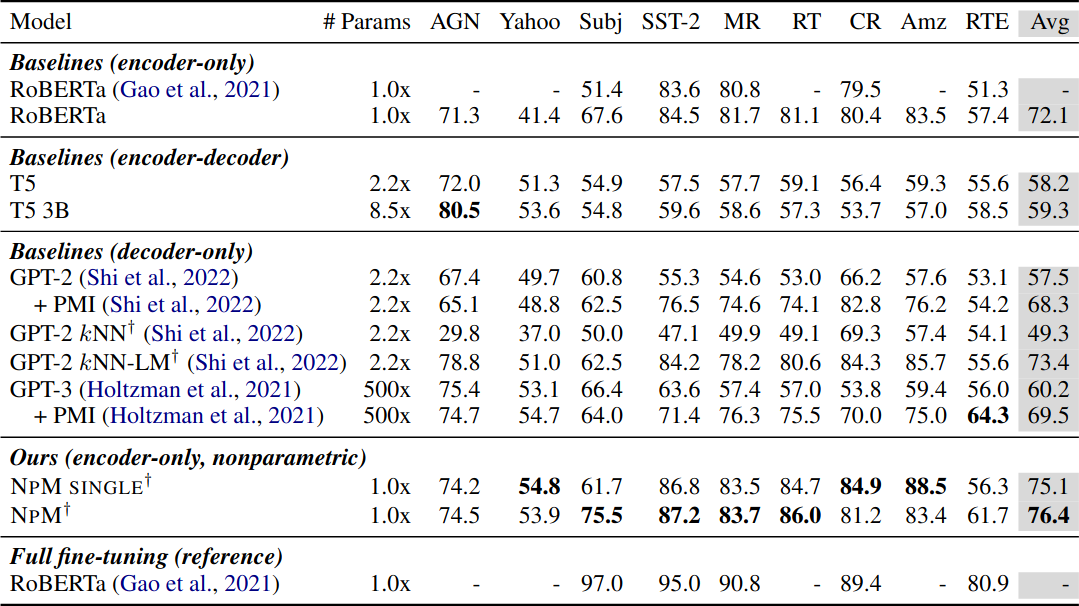
\includegraphics[scale=1.24]{img/npm-scores.png}
    \end{center}
\end{frame}


\begin{frame}
    \frametitle{Other topics}
    \begin{itemize}
        % 5 Oct 2022
        \item \textbf{GLM-130B} \cite{glm_130b} -- bilingual (English and Chinese) pre-trained language model with 130 billion parameters
        % 13 Feb 2023
        \item \textbf{Lion} \cite{lion} -- new optimization algorithm
        % 15 Feb 2023
    	    \item \textbf{ChatRWKV} \href{https://github.com/BlinkDL/ChatRWKV}{[GitHub]} -- ChatRWKV \cite{rwkv} is like ChatGPT but powered by my RWKV (100\% RNN) language model
    	    % 21 Feb 2023
        \item \textbf{Hyena} \cite{hyena} -- subquadratic drop-in replacement for attention constructed by interleaving implicitly parametrized long convolutions and data-controlled gating
        % 27 Feb 2023
    	    \item \textbf{SpikeGPT} \cite{spikegpt} -- generative language model with pure binary, event-driven spiking activation units, inspired by RWKV models
    	    % 27 Feb 2023
    	    \item \textbf{LLaMA} \cite{llama} -- collection of foundation language models ranging from 7B to 65B parameters
    \end{itemize}
\end{frame}

\begin{frame}
    \frametitle{Other topics}
    \begin{itemize}
    	    % 27 Feb 2023
    	    \item \textbf{KOSMOS-1} \cite{kosmos} -- Multimodal Large Language Model (MLLM) t trained on web-scale multi-modal corpora, including arbitrarily interleaved text and images, image-caption pairs, and text data
    	    % 6 March 2023
    	    \item \textbf{PaLM-E} \cite{palme} -- fine-tune PaLM on multiple embodied tasks including sequential robotic manipulation planning, visual question answering, and captioning
        % 2 Mar 2023
    	    \item \textbf{ParaFormer} \cite{paraformer} -- fast and accurate parallel transformer
    	    % 2 Mar 2023
    	    \item \textbf{Dropout} \cite{dropout} -- early dropout and late dropout
    	    \item \textbf{huggingface.js} \href{https://github.com/huggingface/huggingface.js}{[GitHub]} -- JS libraries to interact with the Hugging Face API, with TS types included
    	    \item \textbf{pandas 2.0} and the Arrow revolution \href{https://datapythonista.me/blog/pandas-20-and-the-arrow-revolution-part-i}{[datapythonista blog]}
    \end{itemize}
\end{frame}

\begin{frame}
    \frametitle{Unifying Language Learning Paradigms (UL2)}
    \begin{itemize}
    	    \item \textbf{UL2} (T5 UL2/FLAN-UL2) - release FLAN-UL2 20B \href{https://github.com/google-research/google-research/tree/master/ul2}{[GitHub]}
    \end{itemize}
    \begin{center}
        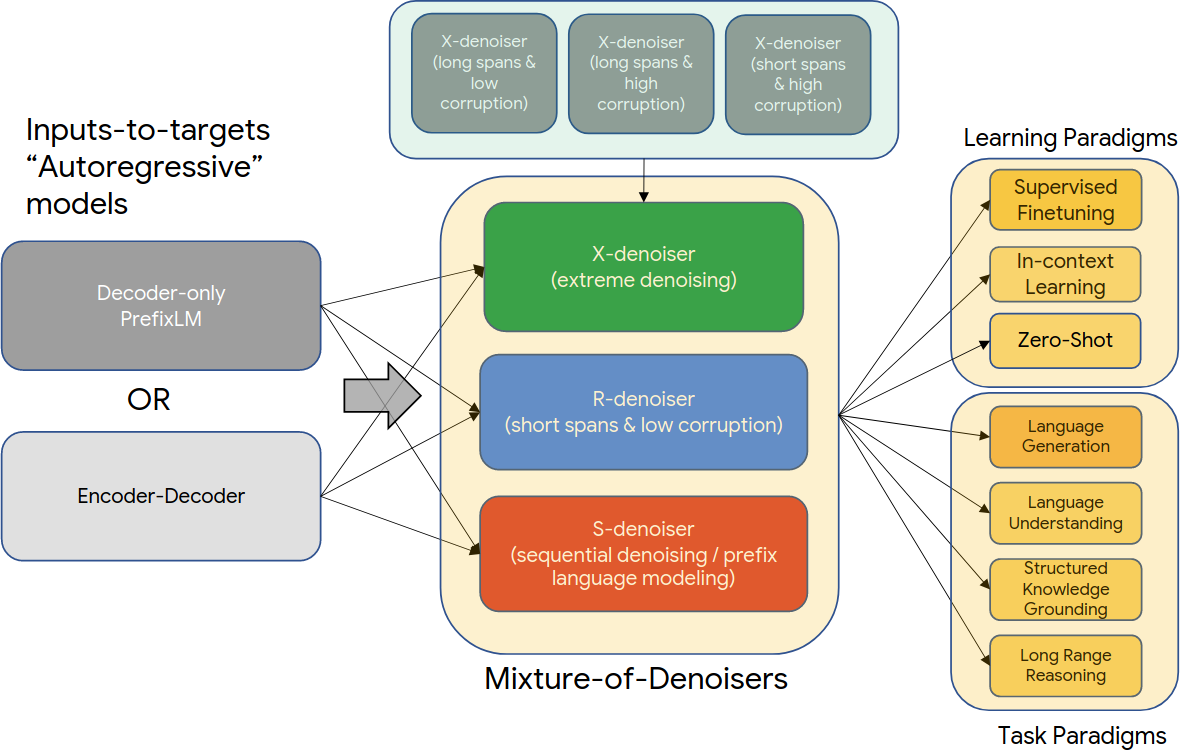
\includegraphics[scale=0.95]{img/ul2.png}
    \end{center}
\end{frame}

\begin{frame}
    \frametitle{Unifying Language Learning Paradigms (UL2)}
    \begin{center}
        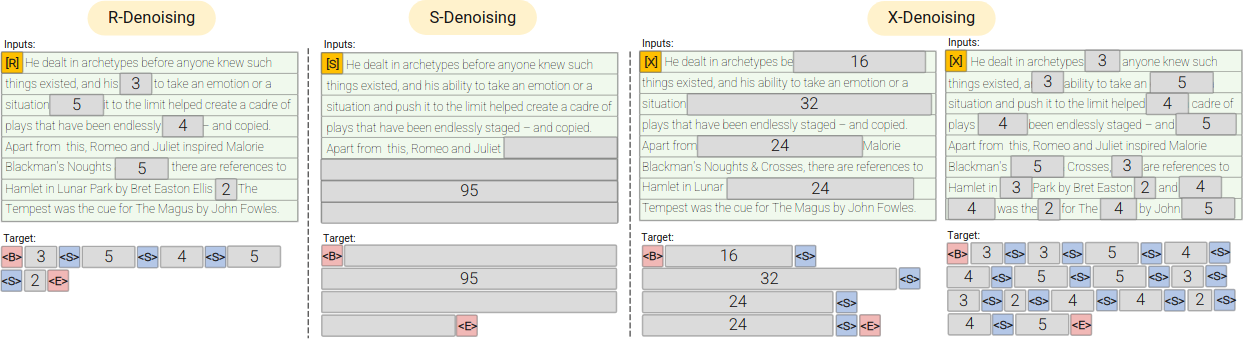
\includegraphics[scale=1.1]{img/ul2_masking.png}
    \end{center}
\end{frame}


\begin{frame}
    \frametitle{Some of my future}
    \begin{columns}
    \begin{column}{0.5\textwidth}
    \footnotesize
    \begin{itemize}
        \item checking if there is a correlation between \textbf{pre-trained model "loss"} and \textbf{downstream task}
        \item tested models base on Transformer architecture (encoder, decoder, encoder-decoder) -- check $\sim$60 models
        \item not all models are available -- they are not released
        \item not all models can be used -- some weights missing or are too big
        \item training some models are not trivial -- fast training is not trivial!
        \item make sure all experiments are easy do reproduce
    \end{itemize}
    \end{column}
    \begin{column}{0.5\textwidth}
    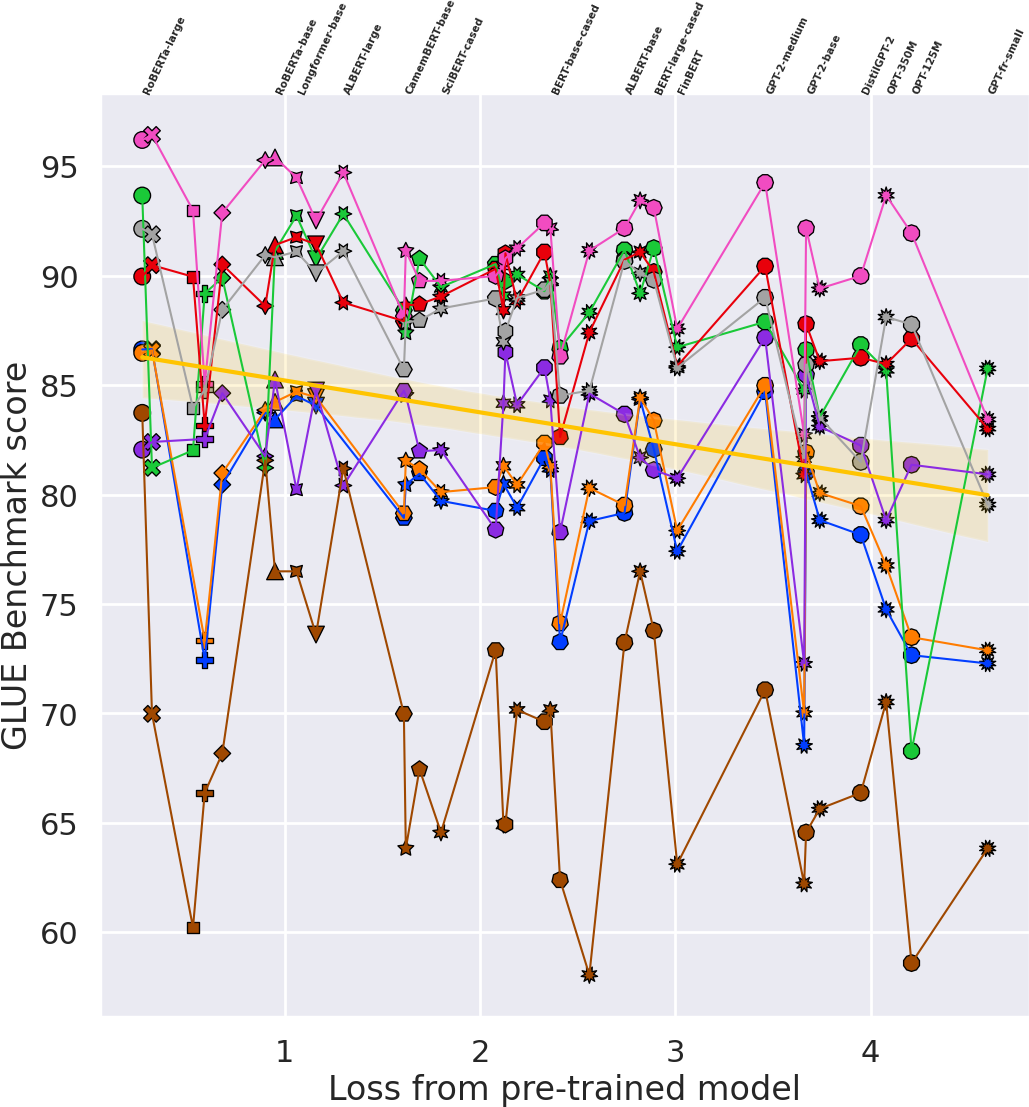
\includegraphics[scale=0.2]{img/kk-plot-loss.png}
    \end{column}
    \end{columns}
\end{frame}


% References
\section{References}
\begin{frame}[allowframebreaks,t]
    \tiny
    \frametitle{References}
    \bibliographystyle{ieeetr}
    \bibliography{npm}
    %\nocite{*}
\end{frame}

\end{document}
